\documentclass[a4paper, 14pt]{extarticle}
\usepackage{enumitem}
\usepackage{fefutitle}
\usepackage{listings}
\usepackage{xcolor}
\usepackage{amsmath}
\usepackage{amssymb}
\usepackage{graphicx}
\usepackage[justification=centering]{caption}
\usepackage{float}

\lstdefinestyle{mystyle}{
	basicstyle={\small\ttfamily},
	keywordstyle=\color{orange},
	stringstyle=\color{green},
	basicstyle=\ttfamily\footnotesize,
	breakatwhitespace=false,         
	breaklines=true,                 
	captionpos=b,                    
	keepspaces=true,                 
	numbers=none,                    
	numbersep=5pt,                  
	showspaces=false,                
	showstringspaces=false,
	showtabs=false,                  
	tabsize=2,
	aboveskip=3mm,
	belowskip=3mm,
}
\lstset{style=mystyle}

\begin{document}
	\fefutitle{1}
	\pagebreak	

	\section{Постановка задачи}
		Минимизировать функцию $ f(x) = \dfrac{1}{2} \cdot x^TAx + b \cdot x$
		
		$A_{6\times6}$ - произвольная положительно определенная матрица, $A \in \mathbb{R}^{6\times6}$
		
		$b$	- произвольный ненулевой вектор размерности 6, $b \in \mathbb{R}^{6\times1}$ 
		
		$x_0$ - произвольный начальный ненулевой вектор размера 6, отдаленный от точного решения, $ x \in \mathbb{R}^{6\times1} $
		
		\scalebox{0.9}{$ A = \begin{pmatrix}
				3.5250663 & 3.47620458 & 3.48870342 & 3.25241547 & 3.13102997 & 2.8216509\\
				3.47620458 & 3.67981631 & 3.58848911 & 3.3682241 & 3.07763483 & 2.89993938\\
				3.48870342 & 3.58848911 & 3.64737011 & 3.35467961 & 3.04393178 & 2.84412883\\
				3.25241547 & 3.3682241 & 3.35467961 & 3.22609546 & 2.86574917 & 2.71725572\\
				3.13102997 & 3.07763483 & 3.04393178 & 2.86574917 & 2.87270201 & 2.5177417\\
				2.8216509 & 2.89993938 & 2.84412883 & 2.71725572 & 2.5177417 & 2.34092264\\		
			\end{pmatrix}$}
		
		$ \lambda_1 = 18.8098291,\, \lambda_2 = 0.272692101,\, \lambda_3 = 0.00307129084,\, \lambda_4 = 0.0250115652,\,\\ \lambda_5 = 0.103202992,\, \lambda_6 = 0.0781657514 \Rightarrow $ $A$ - положительно определенная
		
		$b = \begin{pmatrix} 
				1.36886891\\
				1.20398408\\
				1.61577703\\
				1.64312545\\
				1.65507064\\
				1.22275572
			\end{pmatrix}  $
		
		$x_0 = \begin{pmatrix} 
			16.19429902
			11.92643976\\
			-11.19044284\\
			1.40865507\\
			-9.68338119\\
			-12.59783428
		\end{pmatrix}  $		
	
	\section{Метод градиента}
		$x_{k+1} = x_k - \lambda f'(x_k)$, где $\lambda = 10^{-4}$
		
		Первая производная функции: $ f'(x) = \dfrac{1}{2}\big(A^T + A\big)x + b $
		
		Присваивая производную к нулю, получаем вектор $x_{\text{точ}} \in \mathbb{R}^{6\times1}$
		
		$x_{\text{точ}} = \begin{pmatrix}
			12.45715309\\
			 9.17418443\\
			-8.60803295\\
			 1.08358083\\
			-7.44875477\\
			-9.69064175
		\end{pmatrix}$
	
		$f_{\text{точ}} = -4.10396203$
		
		 Алгоритм отработал за 9 324 шагов. Условие выхода из цикла: $ || x_{k+1} - x_k || < \xi = 10^{-5} $
		 
		\textit{Промежуточные результаты:}
		 
		 $x_{\frac{m}{4}} = \begin{pmatrix}
		 	16.10199799\\
		 	 11.73362197\\
		 	-11.10667036\\
		 	  1.56282895\\
		 	 -9.47432949\\
		 	-12.59381325
		 \end{pmatrix} $
	 
		 $x_{\frac{m}{2}} = \begin{pmatrix}
		 	15.97377011\\
		 	11.5578125\\
		 	-11.03759348\\
		 	1.68277894\\
		 	-9.32233186\\
		 	-12.60833778
		 \end{pmatrix} $
	 
	 $x_{\frac{3m}{2}} = \begin{pmatrix}
	 	 15.8420995 \\
	 	 11.41250677\\
	 	-10.96519231\\
	 	  1.78884126\\
	 	 -9.19159334\\
	 	-12.62155374
	 \end{pmatrix} $
 
	 $x_{m} = \begin{pmatrix}
	 	15.71141566\\
	 	11.2904892\\
	 	-10.89287998\\
	 	1.88073392\\
	 	-9.07461642\\
	 	-12.6334531
	 \end{pmatrix} $
	\pagebreak
	
 	\textit{Промежуточные значения функционала:}
 	
 		$f\big(x_{\frac{m}{4}}\big) = -3.81507671$
 		
 		$f\big(x_{\frac{m}{2}}\big) = -3.85368977$
 		
 		$f\big(x_{\frac{3m}{4}}\big) = -3.88470915$
 		
 		$f\big(x_m) = -3.91025668$
 		
 	\textit{Погрешности метода градиента:}
 	
 	$x_{\text{точ}} = \begin{pmatrix}
			12.45715309\\
			9.17418443\\
			-8.60803295\\
			1.08358083\\
			-7.44875477\\
			-9.69064175
		\end{pmatrix}$
	$x_{m} = \begin{pmatrix}
		15.71141566\\
		11.2904892\\
		-10.89287998\\
		1.88073392\\
		-9.07461642\\
		-12.6334531
	\end{pmatrix}$
	
 	$|x_{m1} - x_{\text{точ}}| = 3.25426257$
 	
 	$|x_{m2} - x_{\text{точ}}| = 2.11630477$
 	
 	$|x_{m3} - x_{\text{точ}}| = 2.28484703$
 	
 	$|x_{m4} - x_{\text{точ}}| = 0.79715309$
 	
 	$|x_{m5} - x_{\text{точ}}| = 1.62586165$
 	
 	$|x_{m6} - x_{\text{точ}}| = 2.94281135$
 	
 	$|f(x_m) - f(x_{\text{точ}})| = 0.19370535$
 	
 	\begin{figure}[H]
 		\centering
 		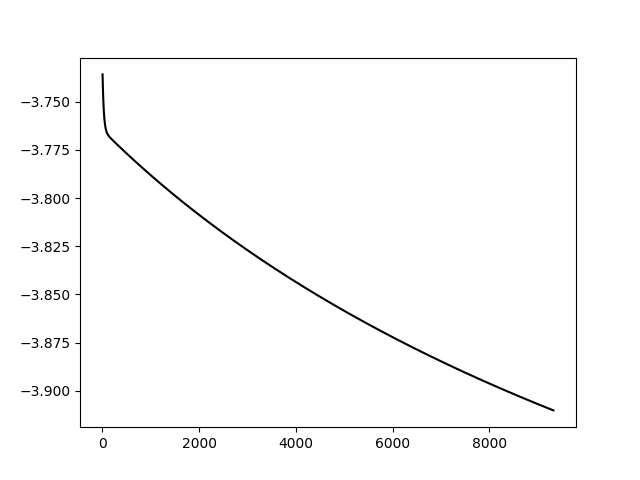
\includegraphics[width = \linewidth]{fig1.png}
 		\caption[.] {График зависимости значения функции от номера шага методом градиентного спуска }
 	\end{figure}
 	Алгоритм содержится в приложении 1.
 	
 	\section{Приложения}
 	\begin{lstlisting}[language=python]
import numpy as np
import matplotlib.pyplot as plt


def generate_pd_matrix(n: int, m: int) -> np.ndarray:
	matrix = np.random.uniform(0.5, 1, (n, m))
	return np.matmul(matrix, matrix.transpose())


def f(x: np.ndarray, a: np.ndarray, b: np.ndarray) -> np.ndarray:
	return .5 * x.transpose() @ a @ x + b.transpose() @ x


def f_derivative(a: np.ndarray, b: np.ndarray, x: np.ndarray) -> np.ndarray:
	return .5 * np.matmul(np.add(a.transpose(), a), x) + b


def gradient_descent(a: np.ndarray, b: np.ndarray, initial_x: np.ndarray, h=10e-4, precision=10e-5):
	counter = 0
	res_tuples = []
	error = float('inf')
	prev = None
	current = initial_x
	while error >= precision:
		prev = current
		current = np.subtract(prev, h * f_derivative(a, b, prev))
		error = np.linalg.norm(np.subtract(current, prev), 'fro')
		counter += 1
		res_tuples.append((counter, current))
	return res_tuples


if __name__ == '__main__':
	matrix_a = np.loadtxt("matrix_a.txt", usecols=range(6))
	vector_b = np.loadtxt("vector_b.txt", usecols=range(1), ndmin=2)
	x_sol = np.linalg.solve(.5 * np.add(matrix_a.transpose(), matrix_a), -vector_b)
	vector_x0 = x_sol * -2
	
	ans = gradient_descent(matrix_a, vector_b, vector_x0)
	f_values = np.ravel([f(i[1], matrix_a, vector_b).flatten() for i in ans]).tolist()
	plt.plot([i[0] for i in ans], f_values, 'black')
	plt.savefig('fig1.png')	
 	\end{lstlisting}
		  
\end{document}	